\PassOptionsToPackage{hyphens}{url}
\documentclass[11pt]{article}
\usepackage[preprint]{acl}
\usepackage{times}
\usepackage{latexsym}
\usepackage[T1]{fontenc}
\usepackage[utf8]{inputenc}
\usepackage{microtype}
\usepackage{inconsolata}
\usepackage{booktabs}
\usepackage{multirow}
\usepackage{amsmath,amssymb}
\usepackage{graphicx}
\usepackage{tikz}
\usepackage{pifont}
\usepackage{booktabs}
\usepackage{tabularx}
\newcommand{\cmark}{\ding{51}}
\newcommand{\xmark}{\ding{55}}
\newcommand{\task}[1]{\texttt{#1}}
% ---- Every number in the paper is defined here, once. Sources: swebench_pro_v2_2_analysis/ ----
% Dataset
\newcommand{\nTasks}{642}
\newcommand{\nRepos}{11}
\newcommand{\nPublic}{731}
\newcommand{\nDropped}{89}
% Release validation
\newcommand{\oracleVtwoone}{642/642}
\newcommand{\oracleShipped}{619/642}
\newcommand{\oracleRepaired}{642/642}
\newcommand{\nopBoth}{0/642}
\newcommand{\nParserTasks}{48}
\newcommand{\nParserFail}{23}
\newcommand{\nElementWeb}{52}
\newcommand{\nMissingNames}{124}
\newcommand{\nCollapsedNames}{83}
\newcommand{\nClarif}{35}
\newcommand{\nClarifTests}{16}
\newcommand{\nEnvFix}{10}
\newcommand{\nConfigDrops}{3}
% Data facts
\newcommand{\nEmptyPtoP}{313}
\newcommand{\pctEmptyPtoP}{48.8}
\newcommand{\nBasePassFtoP}{314}
\newcommand{\nBasePassTasks}{26}
\newcommand{\nFtoPTotal}{8{,}919}
\newcommand{\nPyLiteral}{511}
\newcommand{\nOfflineOK}{610}
\newcommand{\nNeedNet}{32}
\newcommand{\nNeedNetGo}{27}
\newcommand{\nNeedNetNpm}{3}
\newcommand{\nNeedNetHttp}{2}
% Instruction correction (v2.0 review)
\newcommand{\nCorrected}{69}
\newcommand{\nCorrectedEdited}{68}
\newcommand{\nSetAside}{17}
\newcommand{\nSetAsideOneCause}{14}
% Leakage
\newcommand{\leakFull}{42.9}
\newcommand{\leakStripped}{4.6}
\newcommand{\leakNamedAll}{127}
\newcommand{\leakNamedAllOf}{524}
% Anti-cheating, v2.1 open run (Opus 5 + Claude Code)
\newcommand{\netTrajOpen}{32}
\newcommand{\netOwnRepoOpen}{25}
\newcommand{\netFixShaOpen}{4}
\newcommand{\webFetchTrajOpen}{13}
\newcommand{\webFetchOwnOpen}{11}
\newcommand{\netTrajOpenPct}{5.0}
% Anti-cheating, locked run
\newcommand{\netAttemptsLocked}{21}
\newcommand{\netTasksLocked}{11}
\newcommand{\webFetchLocked}{0}
% Probe
\newcommand{\probeImages}{642}
\newcommand{\probeUntracked}{14}
% Results
\newcommand{\opusOldOpen}{50.4}
\newcommand{\opusOpenResolved}{603/642}
\newcommand{\opusOpenPct}{93.9}
\newcommand{\opusOpenErrors}{1}
\newcommand{\glmOpenResolved}{564/642}
\newcommand{\glmOpenPct}{87.9}
\newcommand{\glmOpenErrors}{16}
\newcommand{\opusLockedInplace}{631/642}
\newcommand{\opusLockedRegraded}{631/642}
\newcommand{\opusLockedPct}{98.3}
\newcommand{\nFlips}{4}
\newcommand{\nFails}{11}
\newcommand{\nFailOneTest}{7}
\newcommand{\nFailFixture}{1}
\newcommand{\nFailForgery}{1}
\newcommand{\nFailUI}{1}
\newcommand{\nAgentTimeouts}{1}
\newcommand{\glmLockedResolved}{612/642}
\newcommand{\glmLockedPct}{95.3}
\newcommand{\glmNetAttempts}{61}
\newcommand{\glmNetTasks}{41}
\newcommand{\glmMedSteps}{57}
\newcommand{\glmMedMinutes}{13.8}
\newcommand{\glmFails}{30}
\newcommand{\glmFailsShared}{4}
\newcommand{\glmTimeouts}{4}
% Behaviour / cost
\newcommand{\costTotal}{\$912}
\newcommand{\costTask}{\$1.0}
\newcommand{\costFailMult}{2--4$\times$}
\newcommand{\medSteps}{25}
\newcommand{\medMinutes}{5}
\newcommand{\medInputTokens}{0.99\,M}
\newcommand{\cachePct}{97}
\newcommand{\pctRanTests}{97}
\newcommand{\pctPatchTests}{79}
\newcommand{\pctHiddenTestFiles}{75}
\newcommand{\pctSymbolsVerbatim}{60}
\newcommand{\pctSymbolsNamed}{38}
\newcommand{\passNamedAll}{100.0}
\newcommand{\nNamedAll}{120}
\newcommand{\passNotAll}{97.5}
\newcommand{\nNotAll}{443}
\newcommand{\phaseExplore}{46}
\newcommand{\phaseEdit}{27}
\newcommand{\phaseTest}{15}
% SWE-Bench Pro Verified (arXiv 2609.08149)
\newcommand{\verTasks}{731}
\newcommand{\verRefined}{102}
\newcommand{\verPassFail}{186}
\newcommand{\verHackAttrib}{169}
\newcommand{\verGLMBase}{78.80}
\newcommand{\verGLMAnti}{57.32}
\newcommand{\verGLMVer}{59.51}
\newcommand{\verDSBase}{49.98}
\newcommand{\verDSAnti}{49.11}
\newcommand{\verDSVer}{49.93}
\newcommand{\verKimi}{62.93}
\newcommand{\verGPT}{61.97}
\newcommand{\verGLMfive}{58.82}
% Prior internal intervention matrix (Opus 4.7, unpublished)
\newcommand{\specIssueOnly}{21}
\newcommand{\specFull}{56}
% Teleport ablation
\newcommand{\ablGolden}{1.98}
\newcommand{\ablCancel}{1.01}
\newcommand{\ablRevert}{10.01}

% ---- Revision (post review) ----
\newcommand{\ciOpusLo}{97.0}
\newcommand{\ciOpusHi}{99.0}
\newcommand{\ciGlmLo}{93.4}
\newcommand{\ciGlmHi}{96.7}
\newcommand{\opusRawRegrade}{630/642}
\newcommand{\glmRawRegrade}{612/642}
\newcommand{\nClarifiedPassOpus}{35}
\newcommand{\nClarifiedPassGlm}{30}
\newcommand{\nNonClar}{607}
\newcommand{\opusNonClar}{596/607}
\newcommand{\opusNonClarPct}{98.2}
\newcommand{\glmNonClar}{582/607}
\newcommand{\glmNonClarPct}{95.9}
\newcommand{\pairedOpusOnly}{26}
\newcommand{\pairedGlmOnly}{7}
\newcommand{\pairedBothFail}{4}
\newcommand{\nRunnerCfgOpus}{12}
\newcommand{\nRunnerCfgGlm}{11}
\newcommand{\nApplyFallback}{28}
\newcommand{\nRegrades}{1{,}284}
\newcommand{\nEmptyPatch}{5}
\newcommand{\nFailIncomplete}{1}
\newcommand{\harborVersion}{0.22.0}
\newcommand{\modalVersion}{1.5.5}
\newcommand{\nTeleportRerun}{38}

% ---- Final revision (2026-09-23): V2 = v2.4 release; multi-system locked runs; Hard-51; private 272 ----
% Release lineage and v2.4 gate
\newcommand{\vtwofourInstr}{231}
\newcommand{\vtwofourImages}{211}
\newcommand{\vtwothreeInstr}{112}
\newcommand{\vtwothreeClarifNew}{54}
\newcommand{\nClarifVtwothree}{89}
\newcommand{\vtwothreeOracleFirst}{637/642}
\newcommand{\vtwothreeDetFails}{3}
\newcommand{\oracleVtwofour}{642/642}
\newcommand{\nopVtwofour}{0/642}
\newcommand{\vtwofourFlakes}{3}
% Human expert effort (instruction correction, public + private sets)
\newcommand{\nEngineers}{23}
\newcommand{\expertHours}{1{,}897}
\newcommand{\medianHoursPerTask}{2}
% Locked v2.4 runs (this paper): in place / fresh raw / fresh adjudicated / % / CI / timeouts
\newcommand{\opusFiveFiveInplace}{638}
\newcommand{\opusFiveFiveRaw}{637}
\newcommand{\opusFiveFiveAdj}{638/642}
\newcommand{\opusFiveFivePct}{99.4}
\newcommand{\ciOpusFiveFiveLo}{98.4}
\newcommand{\ciOpusFiveFiveHi}{99.8}
\newcommand{\opusFiveFiveTimeouts}{0}
\newcommand{\opusXInplace}{637}
\newcommand{\opusXRaw}{637}
\newcommand{\opusXAdj}{638/642}
\newcommand{\opusXPct}{99.4}
\newcommand{\ciOpusXLo}{98.4}
\newcommand{\ciOpusXHi}{99.8}
\newcommand{\opusXTimeouts}{3}
\newcommand{\fableInplace}{635}
\newcommand{\fableRaw}{635}
\newcommand{\fableAdj}{636/642}
\newcommand{\fablePct}{99.1}
\newcommand{\ciFableLo}{98.0}
\newcommand{\ciFableHi}{99.6}
\newcommand{\fableTimeouts}{1}
\newcommand{\astraInplace}{623}
\newcommand{\astraRaw}{622}
\newcommand{\astraAdj}{622/642}
\newcommand{\astraPct}{96.9}
\newcommand{\ciAstraLo}{95.2}
\newcommand{\ciAstraHi}{98.0}
\newcommand{\astraTimeouts}{0}
\newcommand{\astraSetupReruns}{164}
\newcommand{\geminiInplace}{610}
\newcommand{\geminiRaw}{609}
\newcommand{\geminiAdj}{609/642}
\newcommand{\geminiPct}{94.9}
\newcommand{\ciGeminiLo}{92.9}
\newcommand{\ciGeminiHi}{96.3}
\newcommand{\geminiTimeouts}{78}
\newcommand{\geminiTimeoutsPass}{65}
\newcommand{\geminiRouteDev}{91}
\newcommand{\geminiRouteVertex}{551}
\newcommand{\inklingLockedResolved}{530/642}
\newcommand{\inklingLockedPct}{82.6}
\newcommand{\ciInklingLo}{79.4}
\newcommand{\ciInklingHi}{85.3}
\newcommand{\ccVersion}{2.1.278}
\newcommand{\codexVersion}{0.155.1}
% Leaderboard runs under the same protocol (team runs; not re-graded by this paper's replay pass)
\newcommand{\kimiLbResolved}{627/642}
\newcommand{\kimiLbPct}{97.7}
\newcommand{\glmLbResolved}{614/642}
\newcommand{\glmLbPct}{95.6}
\newcommand{\inklingLbResolved}{577/642}
\newcommand{\inklingLbPct}{89.9}
% Flips in the v2.4 runs
\newcommand{\nFlipsOpusFiveFive}{1}
\newcommand{\nFlipsOpusX}{2}
\newcommand{\nFlipsFable}{2}
\newcommand{\nFlipsAstra}{1}
\newcommand{\nFlipsGemini}{5}
\newcommand{\nGeminiForgeries}{3}
% Network audit under lock, v2.4 runs (detected fetch commands / bytes retrieved)
\newcommand{\netOpusX}{28}
\newcommand{\netOpusFiveFive}{9}
\newcommand{\netFable}{46}
\newcommand{\netAstra}{46}
\newcommand{\netBytes}{0}
% Failure audit (Gemini 3.8 Flash, 33 fresh failures)
\newcommand{\auditFails}{33}
\newcommand{\auditOracle}{33/33}
\newcommand{\auditRegrades}{0/66}
\newcommand{\auditOpusPass}{29}
\newcommand{\auditGlmPass}{25}
\newcommand{\auditAllFail}{2}
\newcommand{\auditModel}{23}
\newcommand{\auditBorderline}{7}
\newcommand{\auditDefects}{3}
\newcommand{\geminiExDefects}{609/639}
\newcommand{\geminiExDefectsPct}{95.3}
% Hard-51
\newcommand{\nHard}{51}
\newcommand{\nHardCandidates}{54}
\newcommand{\nHardDefectDrop}{3}
\newcommand{\nHardAuditDrop}{3}
\newcommand{\hardOpusX}{50}
\newcommand{\hardOpusXPct}{98.0}
\newcommand{\hardOpusFiveFive}{49}
\newcommand{\hardOpusFiveFivePct}{96.1}
\newcommand{\hardFable}{47}
\newcommand{\hardFablePct}{92.2}
\newcommand{\hardAstra}{46}
\newcommand{\hardAstraPct}{90.2}
\newcommand{\hardGemini}{30}
\newcommand{\hardGeminiPct}{58.8}
\newcommand{\hardOpusHigh}{40}
\newcommand{\hardOpusHighPct}{78.4}
\newcommand{\hardGlm}{28}
\newcommand{\hardGlmPct}{54.9}
\newcommand{\hardInkling}{6}
\newcommand{\hardInklingPct}{11.8}
\newcommand{\hardInklingVfour}{26}
\newcommand{\hardInklingVfourPct}{51.0}
\newcommand{\hardSonnet}{45}
\newcommand{\hardTerra}{44}
\newcommand{\hardKimi}{44}
\newcommand{\hardGlmLb}{44}
\newcommand{\hardSol}{42}
\newcommand{\hardInklingLb}{16}
\newcommand{\hardHaiku}{13}
\newcommand{\hardGlmPi}{44}
\newcommand{\hardGlmOpencode}{44}
\newcommand{\hardGlmMini}{43}
\newcommand{\hardKimiMini}{45}
\newcommand{\hardKimiPi}{41}
\newcommand{\hardKimiOpencode}{45}
\newcommand{\hardInklingMini}{29}
\newcommand{\hardInklingPi}{21}
\newcommand{\hardInklingOpencode}{32}
% Private set (272 tasks)
\newcommand{\nPriv}{272}
\newcommand{\nPrivOrgs}{4}
\newcommand{\nPrivGo}{154}
\newcommand{\privOpusShipped}{222/272}
\newcommand{\privOpusShippedPct}{81.6}
\newcommand{\privOpusV}{240/272}
\newcommand{\privOpusVPct}{88.2}
\newcommand{\ciPrivOpusLo}{83.9}
\newcommand{\ciPrivOpusHi}{91.5}
\newcommand{\privKimiShipped}{214/272}
\newcommand{\privKimiShippedPct}{78.7}
\newcommand{\privKimiV}{229/272}
\newcommand{\privKimiVPct}{84.2}
\newcommand{\ciPrivKimiLo}{79.4}
\newcommand{\ciPrivKimiHi}{88.0}
\newcommand{\privGeminiShipped}{211/272}
\newcommand{\privGeminiShippedPct}{77.6}
\newcommand{\privGeminiV}{227/272}
\newcommand{\privGeminiVPct}{83.5}
\newcommand{\ciPrivGeminiLo}{78.6}
\newcommand{\ciPrivGeminiHi}{87.4}
\newcommand{\privGlmShipped}{211/272}
\newcommand{\privGlmShippedPct}{77.6}
\newcommand{\privGlmV}{226/272}
\newcommand{\privGlmVPct}{83.1}
\newcommand{\ciPrivGlmLo}{78.2}
\newcommand{\ciPrivGlmHi}{87.1}
\newcommand{\privInklingShipped}{184/272}
\newcommand{\privInklingShippedPct}{67.6}
\newcommand{\privInklingV}{194/272}
\newcommand{\privInklingVPct}{71.3}
\newcommand{\ciPrivInklingLo}{65.7}
\newcommand{\ciPrivInklingHi}{76.4}
\newcommand{\privTimeoutsOpus}{0}
\newcommand{\privTimeoutsKimi}{14}
\newcommand{\privTimeoutsGemini}{31}
\newcommand{\privTimeoutsGlm}{5}
\newcommand{\privTimeoutsInkling}{0}
\newcommand{\privReplays}{1{,}360}
\newcommand{\privAllFail}{20}
\newcommand{\gapShipped}{17.8}
\newcommand{\gapV}{11.2}
\newcommand{\gapVerifier}{6.6}
\newcommand{\privDoneTasksMax}{20}
\newcommand{\privDoneTasksMin}{15}
\newcommand{\privGoRediscover}{59/250}
\newcommand{\privEmptyPtoP}{187}
\newcommand{\privLeak}{59.4}
\newcommand{\privAlignA}{30}
\newcommand{\privAlignB}{107}
\newcommand{\privAlignC}{117}
\newcommand{\privAlignD}{18}
\newcommand{\privUnspec}{65}
\newcommand{\privUnsolvable}{29}
\newcommand{\privAllFailCD}{19}
\newcommand{\privOpusSteps}{31}
\newcommand{\privOpusStepsNinety}{70}
\newcommand{\privOpusTokens}{1.48\,M}
\newcommand{\privOpusRanTests}{229}
\newcommand{\privOpusFetch}{9}
% Cost per task on v2.4 (key-spend deltas)
\newcommand{\costAstra}{\$2.3}
\newcommand{\costGemini}{\$3}
\newcommand{\costClaudeCode}{\$2.9}
% Harness study (team runs, same protocol): models x harnesses
\newcommand{\hsFailMoreTokens}{8 of 9}
% Hard-51 leaderboard percentages
\newcommand{\hardSonnetPct}{88.2}
\newcommand{\hardTerraPct}{86.3}
\newcommand{\hardKimiPct}{86.3}
\newcommand{\hardGlmLbPct}{86.3}
\newcommand{\hardSolPct}{82.4}
\newcommand{\hardInklingLbPct}{31.4}
\newcommand{\hardHaikuPct}{25.5}
% Round-2 review additions
\newcommand{\privOpusAB}{132/137}
\newcommand{\privOpusABPct}{96.4}
\newcommand{\privOpusCD}{108/135}
\newcommand{\privOpusCDPct}{80.0}
\newcommand{\privABLo}{79.6}
\newcommand{\privABHi}{96.4}
\newcommand{\privCDLo}{63.0}
\newcommand{\privCDHi}{80.0}
\newcommand{\privGoFoundOpus}{131}
\newcommand{\privGoFoundInkling}{65}
\newcommand{\glmNonClarDelta}{six tenths}
\newcommand{\opusLockedInplaceN}{631}
\newcommand{\opusRawRegradeN}{630}
\newcommand{\glmLockedN}{612}

% ---- Round-3 revision (2026-09-28): final private set, edit split, paired tests, relay audit ----
% Private final set (same 272 tasks; instructions + images + verifier repaired by the maintainers; locked re-runs)
\newcommand{\privFinalOpus}{253/272}
\newcommand{\privFinalOpusPct}{93.0}
\newcommand{\ciPrivFinalOpusLo}{89.3}
\newcommand{\ciPrivFinalOpusHi}{95.5}
\newcommand{\privFinalKimi}{240/272}
\newcommand{\privFinalKimiPct}{88.2}
\newcommand{\ciPrivFinalKimiLo}{83.9}
\newcommand{\ciPrivFinalKimiHi}{91.5}
\newcommand{\privFinalGlm}{239/272}
\newcommand{\privFinalGlmPct}{87.9}
\newcommand{\ciPrivFinalGlmLo}{83.5}
\newcommand{\ciPrivFinalGlmHi}{91.2}
\newcommand{\privFinalGemini}{234/272}
\newcommand{\privFinalGeminiPct}{86.0}
\newcommand{\ciPrivFinalGeminiLo}{81.4}
\newcommand{\ciPrivFinalGeminiHi}{89.6}
\newcommand{\privFinalInkling}{215/272}
\newcommand{\privFinalInklingPct}{79.0}
\newcommand{\ciPrivFinalInklingLo}{73.8}
\newcommand{\ciPrivFinalInklingHi}{83.5}
% forgery-adjusted (uncaught imitation-SDK passes counted as fail)
\newcommand{\privStrictOpus}{252}
\newcommand{\privStrictOpusPct}{92.6}
\newcommand{\privStrictKimi}{238}
\newcommand{\privStrictKimiPct}{87.5}
\newcommand{\privStrictGlm}{237}
\newcommand{\privStrictGlmPct}{87.1}
\newcommand{\nFakeSDK}{5}
% in-place and flips on the final set
\newcommand{\privFinalInplaceOpus}{255}
\newcommand{\privFinalInplaceKimi}{237}
\newcommand{\privFinalInplaceGlm}{238}
\newcommand{\privFinalInplaceGemini}{220}
\newcommand{\privFinalInplaceInkling}{212}
\newcommand{\privFinalTimeoutsKimi}{15}
\newcommand{\privFinalTimeoutsGlm}{4}
\newcommand{\privFinalTimeoutsGemini}{60}
\newcommand{\privFinalAllFail}{10}
\newcommand{\privFinalAllFailUnspec}{8}
\newcommand{\privFinalOracle}{270/272}
\newcommand{\privFinalReplaySame}{1{,}358/1{,}360}
\newcommand{\gapFinal}{6.4}
\newcommand{\gapRepairTotal}{11.4}
\newcommand{\gapInstrImage}{4.8}
% private before/after on the 68 substantively edited instructions (pooled over five systems)
\newcommand{\nPrivEdited}{68}
\newcommand{\nPrivUnedited}{204}
\newcommand{\privEditedBefore}{193/340}
\newcommand{\privEditedBeforePct}{56.8}
\newcommand{\privEditedAfter}{249/340}
\newcommand{\privEditedAfterPct}{73.2}
\newcommand{\privUneditedBeforePct}{90.5}
\newcommand{\privUneditedAfterPct}{91.4}
\newcommand{\privEditedUp}{73}
\newcommand{\privEditedDown}{17}
\newcommand{\privUneditedUp}{33}
\newcommand{\privUneditedDown}{24}
% private alignment audit before (v7) / after (final)
\newcommand{\privUnspecAssertBefore}{150}
\newcommand{\privUnspecAssertAfter}{61}
\newcommand{\privUnspecTasksAfter}{41}
\newcommand{\privUnsolvableAfter}{8}
\newcommand{\privLeakThreeBefore}{22}
\newcommand{\privLeakThreeAfter}{18}
\newcommand{\privJudgeAgree}{71}
\newcommand{\privAlignFinalAB}{166}
\newcommand{\privAlignFinalCD}{106}
\newcommand{\privFinalOpusAB}{159/166}
\newcommand{\privFinalOpusABPct}{95.8}
\newcommand{\privFinalOpusCD}{94/106}
\newcommand{\privFinalOpusCDPct}{88.7}
\newcommand{\privFinalABLo}{84.3}
\newcommand{\privFinalABHi}{95.8}
\newcommand{\privFinalCDLo}{70.8}
\newcommand{\privFinalCDHi}{88.7}
% public: tasks whose instruction was edited after v2.2r (v2.3 + v2.4)
\newcommand{\nPubEdited}{229}
\newcommand{\nPubUnedited}{413}
\newcommand{\opusXUnedited}{409/413}
\newcommand{\opusXUneditedPct}{99.0}
\newcommand{\opusHighFailsEdited}{11/11}
\newcommand{\inklingFailsEdited}{78/229}
\newcommand{\inklingFailsUnedited}{34/413}
% public leakage re-measured on V2 text (same instrument across releases)
\newcommand{\leakVtwotwo}{37.3}
\newcommand{\leakVtwo}{38.4}
\newcommand{\leakProblemOnly}{3.6}
\newcommand{\instrGrowth}{11}
% paired exact McNemar (two-sided), Holm-corrected over the ten pairs of each set
\newcommand{\mcAstraGemini}{0.07}
\newcommand{\mcAstraGeminiHolm}{0.29}
\newcommand{\mcFableAstraHolm}{0.013}
% relay audit of agent tool calls (ten locked runs)
\newcommand{\relayCallsPub}{127{,}321}
\newcommand{\relayCallsPriv}{76{,}094}
\newcommand{\relayGlmMsgs}{14{,}796}
\newcommand{\relayHostTasksPub}{3}
\newcommand{\relayHostTasksPriv}{1}
% OpenAI audit of the public split
\newcommand{\oaiPipelinePct}{27.4}
\newcommand{\oaiHumanN}{249}
\newcommand{\oaiHumanPct}{34.1}
% Hard-51 provenance
\newcommand{\hardKimiOnly}{14}
\newcommand{\hardRewritten}{39}
\newcommand{\otherRewritten}{190/591}
\newcommand{\nSolvedByAny}{642/642}

% ---- Paper polish (2026-10-09): pipeline counts used outside Section 3 (keep in sync with sections/03_method.tex) ----
\newcommand{\nFlagged}{200}
\newcommand{\nFlaggedPct}{27}
\newcommand{\nArtifactFlags}{161}
\newcommand{\nFailureFlags}{54}
\newcommand{\nFailureFlagsNew}{39}
\newcommand{\nRepaired}{66}
\newcommand{\nKept}{45}
\newcommand{\nNeverFlagged}{531}
\newcommand{\nDefective}{149}
\newcommand{\nDefectivePct}{20}
\newcommand{\privEditedGain}{16.4}% = privEditedAfterPct - privEditedBeforePct
% Wilson 95% intervals for the partner runs (computed from the resolved counts above)
\newcommand{\ciKimiLbLo}{96.2}
\newcommand{\ciKimiLbHi}{98.6}
\newcommand{\ciGlmLbLo}{93.8}
\newcommand{\ciGlmLbHi}{97.0}
\newcommand{\ciInklingLbLo}{87.3}
\newcommand{\ciInklingLbHi}{92.0}

\sloppy
\newcommand{\dyz}[1]{\textcolor{red}{[Daniel: #1]}}

\title{SWE-Bench Pro v2: A Cleaner, Harder-to-Game Coding Benchmark}
\author{Soham Dan, Jeff Da, Sanyam Bhutani, Miguel Romero...TBD, ..., Ying Liu, Daniel Yue Zhang}

\begin{document}
\maketitle
\begin{abstract}
Issue-resolution benchmarks have become the primary yardstick for coding agents, yet their scores are only as reliable as the tasks and evaluation harness behind them. We audit SWE-Bench Pro, a widely reported benchmark of long-horizon software engineering tasks, and identify two sources of measurement error. First, \nDefectivePct\% of its public tasks are defective: their specifications omit, contradict or leak what the hidden tests check, or their tests and verifiers misjudge correctness. Second, the standard evaluation protocol is exploitable: agents can retrieve upstream fixes over the network, and in-sandbox grading credits state outside the submitted patch, such as forged dependencies. We present SWE-Bench Pro V2, a \nTasks{}-task benchmark constructed by combining agentic audits with expert adjudication and blind re-implementation, together with a locked protocol that confines agents to the model endpoint and re-grades every patch in a pristine container. On V2, frontier agents approach the ceiling (up to \opusXPct\%) while weaker systems remain clearly separated, and a curated \nHard{}-task Hard split restores headroom, spreading systems from \hardHaikuPct\% to \hardOpusXPct\%. A controlled study on a never-public set shows that the repairs change scores where they are applied: pass rates on corrected tasks rise by \privEditedGain{} points, while the remaining tasks move by less than one point. We release the benchmark, the protocol and per-task grades for every run.
% TODO: add one sentence on the harness comparison (Section 4.6) once finalized.
\end{abstract}

\section{Introduction}

Benchmarks built from real GitHub issues, such as SWE-bench \citep{jimenez2024swebench}, have become the standard way to compare coding agents. SWE-Bench Pro \citep{deng2025swebenchpro} was built to be harder: its tasks come from \nRepos{} repositories, need long changes, and each comes with a written specification and hidden tests. \dyz{please expand}

Two problems have since been found. \dyz{Similar comments as the abstract, here's the paragraph where you should really expand on defining the error buckets we found for this benchmark and how we identified those. You can quote the community findings but that should just be a simple reference.} The first is in the data. OpenAI estimated that about 30\% of the public tasks are broken \citep{openai2026signal}. Some tests check details the instruction never mentions. Some instructions contradict the tests. In both cases a correct solution fails. The second is in the evaluation. Agents could cheat in various ways most easily searching the internet or the repository's git history to find the original fix. \citet{swebenchproverified2026} showed this inflates scores: blocking those routes turned \verPassFail{} passes of one model into failures.

We fix both problems and release the result as SWE-Bench Pro V2. To fix the data, \dyz{same comments as abstract, this reads really trivial. Can you describe the actual pipeline we built to fix the data? should be multi-stages and a combination of agentic checks and manual fixes + QC layer } expert engineers corrected instructions so that they state exactly what the tests check, and a second engineer confirmed each fix by solving the task from the corrected text alone.  To fix the evaluation, the agent may reach only the model endpoint, and its patch is graded again in a fresh container it never touched.

After the fixes, the strongest systems solve almost every task (Figure~\ref{fig:spread}). The full set no longer tells them apart, so we also release a Hard split of \nHard{} tasks, which does. \dyz{ok let's rewrite and expand each paragraph, this reads like notes. Here acknowledge frontier models saturated on full set but gap still remain with laggers. Then talk about Hard split to increase the spread. Then note that this is clean set that serves as great test bed for both frontier and OSS small models.} Our contributions are as follows: \dyz{can add harness analysis later. Why "Results" is a contribution? Let's revise these}

\begin{itemize}\setlength\itemsep{0pt}
\item We release SWE-Bench Pro V2: \nTasks{} tasks, each passing with its reference solution.
\item \textbf{Fixing the data.} \nEngineers{} engineers spent \expertHours{} hours correcting instructions, each fix verified by a blind re-implementation.
\item \textbf{Fixing the evaluation.} A locked protocol blocks all network access except the model endpoint and re-grades every patch in a clean container. No run retrieved external content, and re-grading caught every faked dependency.
\item \textbf{Results.} Frontier systems resolve \geminiPct--\opusXPct\% of V2. On the Hard split however, runs range from 59\% to 98\%.
\item We discuss the importance of SWE Bench Pro v2 despite saturation by frontier models.
\end{itemize}

\begin{figure}[t]
\centering\footnotesize
\resizebox{\columnwidth}{!}{%
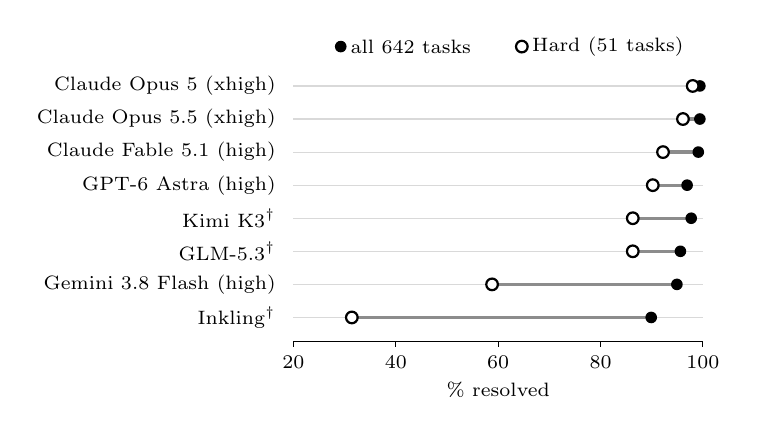
\begin{tikzpicture}
\node[anchor=east,font=\scriptsize] at (-0.1,0.00) {Claude Opus 5 (xhigh)};
\draw[gray!30] (0,0.00) -- (5.2,0.00);
\draw[line width=1.2pt,black!45] (5.070,0.00) -- (5.161,0.00);
\fill[black] (5.161,0.00) circle (2.1pt);
\draw[black,fill=white,line width=0.8pt] (5.070,0.00) circle (2.1pt);
\node[anchor=east,font=\scriptsize] at (-0.1,-0.42) {Claude Opus 5.5 (xhigh)};
\draw[gray!30] (0,-0.42) -- (5.2,-0.42);
\draw[line width=1.2pt,black!45] (4.946,-0.42) -- (5.161,-0.42);
\fill[black] (5.161,-0.42) circle (2.1pt);
\draw[black,fill=white,line width=0.8pt] (4.946,-0.42) circle (2.1pt);
\node[anchor=east,font=\scriptsize] at (-0.1,-0.84) {Claude Fable 5.1 (high)};
\draw[gray!30] (0,-0.84) -- (5.2,-0.84);
\draw[line width=1.2pt,black!45] (4.693,-0.84) -- (5.141,-0.84);
\fill[black] (5.141,-0.84) circle (2.1pt);
\draw[black,fill=white,line width=0.8pt] (4.693,-0.84) circle (2.1pt);
\node[anchor=east,font=\scriptsize] at (-0.1,-1.26) {GPT-6 Astra (high)};
\draw[gray!30] (0,-1.26) -- (5.2,-1.26);
\draw[line width=1.2pt,black!45] (4.563,-1.26) -- (4.999,-1.26);
\fill[black] (4.999,-1.26) circle (2.1pt);
\draw[black,fill=white,line width=0.8pt] (4.563,-1.26) circle (2.1pt);
\node[anchor=east,font=\scriptsize] at (-0.1,-1.68) {Kimi K3$^\dagger$};
\draw[gray!30] (0,-1.68) -- (5.2,-1.68);
\draw[line width=1.2pt,black!45] (4.309,-1.68) -- (5.051,-1.68);
\fill[black] (5.051,-1.68) circle (2.1pt);
\draw[black,fill=white,line width=0.8pt] (4.309,-1.68) circle (2.1pt);
\node[anchor=east,font=\scriptsize] at (-0.1,-2.10) {GLM-5.3$^\dagger$};
\draw[gray!30] (0,-2.10) -- (5.2,-2.10);
\draw[line width=1.2pt,black!45] (4.309,-2.10) -- (4.914,-2.10);
\fill[black] (4.914,-2.10) circle (2.1pt);
\draw[black,fill=white,line width=0.8pt] (4.309,-2.10) circle (2.1pt);
\node[anchor=east,font=\scriptsize] at (-0.1,-2.52) {Gemini 3.8 Flash (high)};
\draw[gray!30] (0,-2.52) -- (5.2,-2.52);
\draw[line width=1.2pt,black!45] (2.522,-2.52) -- (4.869,-2.52);
\fill[black] (4.869,-2.52) circle (2.1pt);
\draw[black,fill=white,line width=0.8pt] (2.522,-2.52) circle (2.1pt);
\node[anchor=east,font=\scriptsize] at (-0.1,-2.94) {Inkling$^\dagger$};
\draw[gray!30] (0,-2.94) -- (5.2,-2.94);
\draw[line width=1.2pt,black!45] (0.741,-2.94) -- (4.543,-2.94);
\fill[black] (4.543,-2.94) circle (2.1pt);
\draw[black,fill=white,line width=0.8pt] (0.741,-2.94) circle (2.1pt);
\draw (0,-3.24) -- (5.2,-3.24);
\draw (0.000,-3.24) -- (0.000,-3.31) node[below,font=\scriptsize] {20};
\draw (1.300,-3.24) -- (1.300,-3.31) node[below,font=\scriptsize] {40};
\draw (2.600,-3.24) -- (2.600,-3.31) node[below,font=\scriptsize] {60};
\draw (3.900,-3.24) -- (3.900,-3.31) node[below,font=\scriptsize] {80};
\draw (5.200,-3.24) -- (5.200,-3.31) node[below,font=\scriptsize] {100};
\node[font=\scriptsize] at (2.60,-3.86) {\% resolved};
\fill[black] (0.6,0.5) circle (2.1pt) node[right,font=\scriptsize] {all 642 tasks};
\draw[black,fill=white,line width=0.8pt] (2.9,0.5) circle (2.1pt) node[right,font=\scriptsize] {Hard (51 tasks)};
\end{tikzpicture}}
\caption{Percent of tasks resolved on SWE-Bench Pro V2 (filled dots) and its Hard split (open dots) under the locked protocol. The full set separates these systems by less than 10 points (89.9--99.4\%); the Hard split spreads them from 31.4\% to 98.0\%. $^\dagger$Partner runs under the same protocol (Table~\ref{tab:main}).}
\label{fig:spread}
\end{figure}


\section{Related Work}
\dyz{again these reads like notes or summarized bullets. Can we expand and make them flow well?}
\paragraph{Coding benchmarks.} SWE-bench \citep{jimenez2024swebench} grades a patch by running the tests of the original fix in a clean container. SWE-bench Verified \citep{openai2024verified} had annotators filter out tasks with unclear specifications or unfair tests. Later benchmarks extend the format to more languages, newer issues and other task sources \citep{zan2025multiswebb,swebenchlive2025,badertdinov2025rebench,miserendino2025swelancer}. SWE-Bench Pro \citep{deng2025swebenchpro} adds long horizon tasks which proved to be significantly more challenging to models at the time of release.

\paragraph{Data Issues. \dyz{these headers are really meaningless, can we change to more informative titles like "Quality Gaps in SWE Benchmarks" or something}} Weak or wrong tests are a known problem \citep{aleithan2024swebenchplus,wang2025solvedissues,utboost2025}, and checklists for rigorous agent benchmarks exist \citep{zhu2025abc}. For SWE-Bench Pro, OpenAI's audit \citep{openai2026signal} found over-strict tests, hidden requirements, narrow tests and misleading instructions. \citet{nadgir2026life} emphasizes that such flaws often surface only once agents are strong enough to reach them.

\paragraph{Reward hacking and leakage.} Agents game tests when they can \citep{zhong2025impossiblebench,gabor2025evilgenie,zhao2026specbench,thaman2026rhb}, and future git history leaked fixes in both SWE-bench and SWE-Bench Pro \citep{kahn2025repostate,needham2025prostate}. Similar to SWE-Bench Pro Verified \citep{swebenchproverified2026}, we block code hosts, hide test files, refine \verRefined{} tasks and checks the refinements with model trial runs. We differ in three ways. We expert verify every instruction and never edit the tests to fit an instruction. We check each fix by a blind human re-implementation. And we grade every patch in a clean second container.

% Preamble: \usepackage{booktabs,tabularx,graphicx,tikz}
%           \usetikzlibrary{positioning,arrows.meta,calc}
\section{Methodology}
\label{sec:method}

We start from the 731 tasks of the original SWE-Bench Pro Public. A task consists of an instruction (problem statement, requirements, new interfaces), a container image with the repository at its base commit, a reference patch, a hidden test patch, fail-to-pass and pass-to-pass lists naming the graded tests, and a verifier that applies the test patch, runs the tests and parses the output. A task is valid if every solution that satisfies the instruction passes and every solution that does not, fails. Our agentic audits flagged 200 tasks (27\%), and engineers adjudicated each flag (Figure~\ref{fig:pipeline}). The released set has 642 tasks: 531 never flagged, 66 repaired and 45 flagged but kept unchanged. The remaining 89 were discarded.

% Pipeline figure for Section~\ref{sec:method}: flow of the 731 tasks.
% Band and bar heights are proportional to task counts (0.046 mm per task).
% Preamble: \usepackage{tikz,graphicx} (xcolor is loaded by tikz)
\definecolor{sbpFlag}{HTML}{4C72B0}
\definecolor{sbpRep}{HTML}{55A868}
\definecolor{sbpDisc}{HTML}{C44E52}
\definecolor{sbpKeep}{HTML}{7F7F7F}
\definecolor{sbpNone}{HTML}{B0B0B0}
\begin{figure*}[t]
\centering
\resizebox{\textwidth}{!}{%
\begin{tikzpicture}[x=1mm, y=1mm, font=\sffamily\scriptsize,
  execute at begin node={\hyphenpenalty=10000\exhyphenpenalty=10000}]
% flagged by an audit
\fill[sbpFlag!22] (2.2,4.09) .. controls (20.1,4.09) and (20.1,8.09) .. (38,8.09)
  -- (38,-1.11) .. controls (20.1,-1.11) and (20.1,-5.11) .. (2.2,-5.11) -- cycle;
% never flagged
\fill[sbpNone!22] (2.2,-5.11) .. controls (20.1,-5.11) and (20.1,-5.11) .. (38,-5.11)
  -- (38,-29.54) .. controls (20.1,-29.54) and (20.1,-29.54) .. (2.2,-29.54) -- cycle;
% discarded
\fill[sbpDisc!22] (40.2,8.09) .. controls (61.1,8.09) and (61.1,11.53) .. (82,11.53)
  -- (82,7.44) .. controls (61.1,7.44) and (61.1,4) .. (40.2,4) -- cycle;
% repaired
\fill[sbpRep!22] (40.2,4) .. controls (61.1,4) and (61.1,4.94) .. (82,4.94)
  -- (82,1.9) .. controls (61.1,1.9) and (61.1,0.96) .. (40.2,0.96) -- cycle;
% kept unchanged
\fill[sbpKeep!22] (40.2,0.96) .. controls (61.1,0.96) and (61.1,-0.6) .. (82,-0.6)
  -- (82,-2.67) .. controls (61.1,-2.67) and (61.1,-1.11) .. (40.2,-1.11) -- cycle;
% never flagged, passes review
\fill[sbpNone!22] (40.2,-5.11) .. controls (81.1,-5.11) and (81.1,-5.11) .. (122,-5.11)
  -- (122,-29.54) .. controls (81.1,-29.54) and (81.1,-29.54) .. (40.2,-29.54) -- cycle;
% repaired -> release
\fill[sbpRep!22] (84.2,4.94) .. controls (103.1,4.94) and (103.1,0) .. (122,0)
  -- (122,-3.04) .. controls (103.1,-3.04) and (103.1,1.9) .. (84.2,1.9) -- cycle;
% kept -> release
\fill[sbpKeep!22] (84.2,-0.6) .. controls (103.1,-0.6) and (103.1,-3.04) .. (122,-3.04)
  -- (122,-5.11) .. controls (103.1,-5.11) and (103.1,-2.67) .. (84.2,-2.67) -- cycle;
% nodes
\fill[black!70] (0,-29.54) rectangle (2.2,4.09);
\fill[sbpFlag] (38,-1.11) rectangle (40.2,8.09);
\fill[sbpNone] (38,-29.54) rectangle (40.2,-5.11);
\fill[sbpDisc] (82,7.44) rectangle (84.2,11.53);
\fill[sbpRep] (82,1.9) rectangle (84.2,4.94);
\fill[sbpKeep] (82,-2.67) rectangle (84.2,-0.6);
\fill[sbpRep] (122,-3.04) rectangle (124.2,0);
\fill[sbpKeep] (122,-5.11) rectangle (124.2,-3.04);
\fill[sbpNone] (122,-29.54) rectangle (124.2,-5.11);
% labels
\node[anchor=east, align=right] at (-1.2,-12.72) {\textbf{731}\\tasks};
\node[anchor=south west, inner sep=1pt] at (38,8.69) {\textbf{200} flagged};
\node[anchor=west] at (68,-17.32) {\textbf{531} never flagged};
\node[anchor=west, inner sep=1pt] at (85.2,9.48) {\textbf{89} discarded};
\node[anchor=west, inner sep=1pt] at (85.2,3.42) {\textbf{66} repaired};
\node[anchor=west, inner sep=1pt] at (85.2,-1.64) {\textbf{45} kept};
\node[anchor=south west, inner sep=1pt] at (122,0.6) {\textbf{642} released};
% stage headers
\node[anchor=north west, inner sep=0pt, text width=34mm, align=left] at (0,25.03)
  {{\bfseries Input}\\[1.5pt]\textcolor{black!65}{SWE-Bench Pro\\Public v1.1}};
\node[anchor=north west, inner sep=0pt, text width=43mm, align=left] at (38,25.03)
  {{\bfseries Agentic audits}\\[1.5pt]\textcolor{black!65}{artifact audit (161 flagged)\\failure audit (54 flagged; 39 new)}};
\node[anchor=north west, inner sep=0pt, text width=38mm, align=left] at (82,25.03)
  {{\bfseries Engineer review}\\[1.5pt]\textcolor{black!65}{verdict on every flag\\blind check of every repair}};
\node[anchor=north west, inner sep=0pt, text width=30mm, align=left] at (122,25.03)
  {{\bfseries Release}\\[1.5pt]\textcolor{black!65}{verifier hardened\\for all tasks}};
\end{tikzpicture}}%
\caption{Flow of the 731 tasks; bar and band heights are proportional to
task counts. The artifact audit (an LLM agent and a human auditor compare the
instruction with the tests and reference patch) and the failure audit (an LLM
judge attributes failed runs of four agent setups) flag 200 tasks. Engineers
adjudicate every flag, and a repair ships only after a blind re-implementation
of the edited instruction passes the hidden tests.}
\label{fig:pipeline}
\end{figure*}


\subsection{Agentic audits}
\label{sec:audits}

\paragraph{Artifact audit.}
An LLM agent compared each task's instruction with its test patch, graded-test lists and reference patch, without executing anything. It flagged six patterns: test requirements missing from the instruction, instruction statements contradicted by the tests, test or solution detail copied into the instruction, changed behaviour that no graded test exercises, fixtures read by the tests but never created, and graded lists naming a whole test file. Requirement sections far above the dataset median length (about 2{,}800 characters) were treated as a leakage signal, as they often transcribed the reference patch. A human auditor reviewed the agent's flags, and marked high-priority cases. The final audit flagged 161 tasks. 

\paragraph{Failure audit.}
We ran four agent configurations on every task: Claude Code with Claude Opus~5, Codex with GPT-5.6, and mini-SWE-agent with each model. For each failed run, an LLM judge read the trajectory, patch, verifier log and graded tests and attributed the failure to the model or to the task. A task was flagged when a patch consistent with a reasonable reading of the instruction was rejected. In one \textit{vuls} task, two configurations fell back to the bundle directory name as instructed and reported \texttt{Sample.app}, while the graded test expects \texttt{Sample} because the reference patch strips the suffix without the instruction saying so. For each flag the judge recorded the defect type, the fix location (instruction, tests, image, graded list or verifier), an effort estimate, a proposed edit, and the passing and failing configurations.
% CHECK: confirm with the audit team that failure attribution was done by an LLM judge.

\subsection{Defect taxonomy}
\label{sec:taxonomy}

We merged the audits' labels into the six categories of Table~\ref{tab:repairs-discards} and assigned each task the defect that determined its outcome. Unstated requirements, contradictions and verifier or environment defects make correct solutions fail. Leakage and insufficient tests make a task easier than intended or let an incomplete solution pass. Table~\ref{tab:problems} maps the categories to data and evaluation problems.

\begin{table}[t]
\centering
\small
\setlength{\tabcolsep}{3pt}
\begin{tabularx}{\columnwidth}{@{}>{\raggedright\arraybackslash}p{2.05cm} >{\raggedright\arraybackslash}X r r@{}}
\toprule
\textbf{Category} & \textbf{Description} & \textbf{Rep.} & \textbf{Disc.} \\
\midrule
Solution leakage & The instruction gives away test or solution detail. & 24 & 4 \\
\addlinespace
Spec--test contradiction & The instruction contradicts what the tests check. & 8 & 5 \\
\addlinespace
Unstated test requirement & The tests require behaviour, names or files the instruction never states. & 31 & 22 \\
\addlinespace
Insufficient tests & The tests miss part of the change or check incidental details instead of behaviour. & 3 & 33 \\
\addlinespace
Verifier or environment defect & The grading setup or container decides the score regardless of the solution. & 0 & 19 \\
\addlinespace
Miscellaneous & -- & -- & 6 \\
\midrule
\textbf{Total} & & \textbf{66} & \textbf{89} \\
\bottomrule
\end{tabularx}
\caption{Defect categories of tasks repaired and kept (Rep.) and discarded (Disc.) between the 731 tasks of SWE-Bench Pro Public v1.1 and the final 642. Repairs edited the instruction in 63 tasks and the test patch in 4 (one task both).}
\label{tab:repairs-discards}
\end{table}

% Needs: \usepackage{booktabs,tabularx}
\begin{table}[t]
\centering\footnotesize
\setlength{\tabcolsep}{3pt}
\begin{tabularx}{\columnwidth}{@{}>{\raggedright\arraybackslash}p{2.05cm}>{\raggedright\arraybackslash}X>{\raggedright\arraybackslash}X@{}}
\toprule
\textbf{Problem} & \textbf{Evidence} & \textbf{Fix} \\
\midrule
\multicolumn{3}{@{}l}{\textit{Data}} \\
Instruction and tests disagree & 94 tasks (Table~\ref{tab:repairs-discards}) & 63 instructions edited; 31 tasks discarded \\
\addlinespace[1.5pt]
Tests too weak & 36 tasks & 3 assertions added; 33 tasks discarded \\
\addlinespace[1.5pt]
Grading or image broken & 19 tasks; shared defects in 253 Go, 322 Python and 47 jest verifiers & 19 tasks discarded; verifiers scoped, capped, re-parsed \\
\addlinespace[1.5pt]
Parser renamed graded tests & Reference patch failed on \nParserFail{} tasks & Graded names regenerated \\
\addlinespace[1.5pt]
Agent files reach grading & 44 runs zeroed; stale bytecode & Test files, test data and bytecode reset before grading \\
\midrule
\multicolumn{3}{@{}l}{\textit{Evaluation}} \\
Open internet & \netTrajOpen{}/\nTasks{} runs reached code hosts; \netOwnRepoOpen{} fetched their own repository & Only the model endpoint reachable; probed before each run \\
\addlinespace[1.5pt]
Web tools outside the sandbox & \webFetchTrajOpen{}/\nTasks{} runs used web fetch & Disabled \\
\addlinespace[1.5pt]
Grading in the agent's sandbox & A \texttt{python3} wrapper scores an empty patch 1 & Re-graded in a clean container \\
\addlinespace[1.5pt]
Fix in git history & \probeImages{} images checked & Fixing commit absent; probed \\
\bottomrule
\end{tabularx}
\caption{Problems found in SWE-Bench Pro and the v2 fix. Data problems concern the tasks; evaluation problems concern how runs are executed and graded.}
\label{tab:problems}
\end{table}

\paragraph{Unstated test requirement (31 repaired, 22 discarded).}
The tests depend on behaviour, names or files the instruction does not mention. In a \textbf{flipt} task, \texttt{TestLoad} reads three YAML samples (\texttt{otlp.yml} with \texttt{samplingRatio} set to 0.5, \texttt{wrong\_sampling\_ratio.yml} and \texttt{wrong\_propagator.yml}) that existed only in the reference patch. The repaired instruction specifies all three. The \textit{vuls} bundle-name task was repaired by stating that the \texttt{.app} suffix is removed. We repaired a task when the missing requirement is behaviour the task is about, and discarded it when the test checks how the reference patch happens to be written, since stating that would give the solution away. Discarded tests read a private attribute (\texttt{\_values} in \textit{qutebrowser}), pin avatar CSS classes in a snapshot (element-web), or inspect a private client through \texttt{reflect} and \texttt{unsafe} (flipt). 

\paragraph{Spec--test contradiction (8 repaired, 5 discarded).}
A vuls instruction said a package is \textit{not affected} when exactly one of the package and the OVAL definition carries a modularity label. Four pre-existing graded cases require the legacy fallback to the host's enabled modules, which the reference patch keeps, and the repair states that fallback. Contradictions whose fix lies in the tests were discarded, for example a \textit{webclients} task whose interface declares an \texttt{Element} argument while the graded test passes a \texttt{Document}.

\paragraph{Solution leakage (24 repaired, 4 discarded).}
Leaky instructions walked through the reference patch file by file, quoted its strings, or copied expected values from the tests. A \textit{tutanota} instruction told the agent to update the try-catch block around \texttt{aes256Decrypt} in \texttt{decrypt}. The repaired version specifies behaviour only: a \texttt{CryptoError} raised by the crypto library must surface as the application's own \texttt{CryptoError}, which the credentials layer converts to \texttt{KeyPermanentlyInvalidatedError}. Repairs delete the leaked text and, where a test depends on it, restate the requirement as behaviour. The four discards were repaired and then removed with a late batch (\S\ref{sec:review}).

\paragraph{Insufficient tests (3 repaired, 33 discarded).}
The graded tests leave part of the change unchecked (28) or assert incidental details (5). In a \textit{flipt} task they cover only the error paths of a new cache layer, so a \texttt{getJSON} that always returns false and a no-op \texttt{setJSON} pass. Engineers did not write tests, so these tasks were discarded. The three repairs are auditor edits that each add one assertion. A \textit{vuls} test now expects an error for an image reference with both a tag and a digest, and a teleport fuzz test now requires the parser error it previously ignored. 

\paragraph{Verifier or environment defect (19 discarded).}
In 16 tasks the fail-to-pass list names a whole file (e.g.\ \texttt{test/tests/calendar/\allowbreak CalendarUtilsTest.js \textbar{} test suite}), so any unrelated or flaky failure in that file fails a correct patch. In 3 tasks the image prevents grading. A vuls test imports a package that exists only in a newer module version than the image's offline Go module cache holds, and a teleport test is skipped because SoftHSM is missing, which the verifier scores as a failure. These tasks needed per-task changes to the graded list or the image, shared verifier defects were fixed globally (\S\ref{sec:verifier}).


\subsection{Engineer review}
\label{sec:review}

Engineers focused on the criteria that if the reference patch adds a behaviour and a hidden test checks it, the instruction must state the behavior, but not how the reference patch implements it. Hidden tests were never edited to agree with an instruction, and instructions were never rewritten to match a wrong test.

23 contracted engineers adjudicated every flag, spending 1{,}897 hours in total. For each claim in a flag they recorded whether it holds, holds in part or does not hold, citing evidence by artifact and line (eg: \texttt{requirements:19}, \texttt{test\_patch\_before:178}, \texttt{f2p:1}, \texttt{golden:562}). A false flag leaves the task unchanged, a flag whose gap is in the instruction leads to an edit limited to where the flag holds, a flag whose remedy lies in the tests, fixtures, verifier or image leads to quarantine, i.e.\ removal. High-priority flags received a second independent review and a third pass by the project team. %The audit team checked all 147 verdicts on its proposed removals and challenged four, which were re-examined.
% CHECK: confirm 23 and 1{,}897 cover the review of all 200 flags, not only the 55 instruction repairs.

For those 147 tasks, reviewers confirmed 70 flags, partly confirmed 21 and rejected 56. The final outcome was 34 repaired, 43 kept and 70 discarded. Of the 54 failure-audit flags, 35 were repaired and 19 discarded. The judge's fix location predicted the outcome well: 28 of the 31 flags it located in the instruction were repaired, and 16 of the 23 located elsewhere were discarded. For the other 7, engineers found a fix, mostly in the instruction (the flipt YAML task is one).

Engineer repairs were validated blind. A second engineer who had seen neither the original task nor the reference patch implemented the edited instruction, and the edit shipped only if that implementation passed the hidden tests. For the auditors' repairs, the reference patch was re-run against the edited tests. Fourteen tasks repaired in a second batch were removed before release, we count them as discards under their original flag, and they include all four leakage discards. Two auditor repairs were not carried into the release, and those tasks are counted as kept. A task counts as repaired only if its instruction or test patch changed in response to a confirmed flag. Release-wide changes are not counted.
% CHECK: add the reason the 14-task batch was removed at release.
% CHECK: the final release also edited instructions of some unflagged tasks and 13 rejected-flag tasks (leak pass); decide whether to disclose these here.

\subsection{Verifier hardening}
\label{sec:verifier}

Defects in shared grading code were fixed for all tasks.

\paragraph{Scoping and resources.}
The Go verifier ran \texttt{go test ./...} over the whole repository. Scoping it to the graded packages on 253 tasks removed out-of-memory failures and timeouts above 150 minutes without changing any grade. Run scripts on 231 tasks that executed the full suite were restricted to the graded tests. With automatic worker counts, pytest-xdist spawned up to 128 workers on small test files and crashed with ``no tests ran'': we capped it at four workers on 239 tasks and inside \texttt{ansible-test} on 83.

\paragraph{Parsing and environment.}
The jest parser assigned tests in failing files to the wrong file and dropped failures (47 tasks), and it truncated test titles at the first parenthesis: it now strips only the trailing timing. We added kernel headers for cgo builds (5 tasks), fetched at grading time one Go module missing from an image's offline cache, re-derived test scoping on 3 tasks that omitted the packages defining the graded tests, and restored CRLF line endings in a fixture that made the reference patch fail.

\paragraph{Test-file reset.}
Before the hidden tests run, the verifier (i)~restores every path the test patch touches and deletes only paths it creates; (ii)~restores modified tracked test data (test data, fixtures, mocks, snapshots), with allowlists for the six reference patches that change fixtures; (iii)~removes agent-written test files that collide with hidden tests; (iv)~clears stale git lock files left by killed agent commands; and (v)~deletes \texttt{\_\_pycache\_\_} and \texttt{.pyc} files. Without (i), agent edits to snapshots owned by the test patch made it fail to apply in 44 runs. Step (v) addresses \texttt{.pyc} files that an agent's \texttt{git stash} round trip left with unchanged size and timestamp, which made the verifier import the base code.

On the assembled 642-task set, the reference patch passes every task and the empty patch fails every task.
% CHECK: re-run the oracle/empty-patch check on the final release package; the 100%/0% result predates the last verifier and instruction updates.

\subsection{Hardened evaluation protocol}
\label{sec:protocol}

We run every model under a locked protocol. The harness sets network access per phase of a run, probes the lock from inside the sandbox before the run starts, and grades the agent's patch in a fresh container rather than in the agent's sandbox. Table~\ref{tab:problems} maps each component to the problem it addresses.

\paragraph{Network.}
With the network open, 32 of 642 Claude Opus~5 trajectories contacted code hosts, and 25 downloaded the task's own repository. Under the lock, the sandbox can reach only the model endpoint during the agent phase; the allowlist names that hostname alone, and the endpoint does not relay other traffic. Web tools that scaffolds execute outside the sandbox are disabled. Before each run, a probe executes in the sandbox under the job's exact flags and aborts the run unless every code host is unreachable, the endpoint answers and the reference patch still passes. The git history of all 642 images contains neither the fixing commit nor any reflog entries, stashes or dangling objects.

\paragraph{Grading.}
The original harness ran the verifier in the sandbox the agent had just used. Because the verifier restores test files but not binaries, a scripted agent that edits no source file and replaces \texttt{python3} with a script printing \textsc{PASSED} scores 1. We saw no model attempt this, but forged dependencies passed through the same gap: with the network closed, some agents that could not fetch a fix edited the Go module cache in place or served a fabricated module version from a local \texttt{GOPROXY}, and neither change appears in the diff. We now save the agent's changes as a patch, apply it to a fresh copy of the task image, run the unchanged verifier there and report that grade. Binaries, module caches, \texttt{node\_modules}, \texttt{site-packages} and \texttt{go env} settings do not carry over.
%We report both grades for every task. When the two disagree, two more fresh grades decide, by majority.
% CHECK: CHEATING_MODES.md says the fresh re-grade is authoritative and that flips are adjudicated with 2 extra fresh re-grades (a forgery fails 2/2, a flake passes at least 1/2). Align the commented sentence with that before re-enabling it.

\paragraph{Audits.}
A fresh re-grade cannot catch a forgery committed inside the patch, so we audit patches for \texttt{replace} directives that point into the patch or to absolute paths, \texttt{go.sum} entries for modules absent from the image, and large new directories that imitate a third-party SDK. We also scan trajectories for fetches that returned content; writes to module caches, package directories or \texttt{/usr/*bin}; and reads of \texttt{/tests} or \texttt{/solution}.
% CHECK: state whether flagged patches are rejected automatically or reviewed by hand.

\section{Experiments}
\label{sec:experiments}

\subsection{Setup}
We run five systems ourselves under the locked protocol of \S\ref{sec:protocol} and report partner runs made under the same protocol (Table~\ref{tab:main}). Claude and GPT models run in their developers' native scaffolds, Claude Code and Codex, with web tools disabled; open-weight models and Gemini run in mini-swe-agent \citep{minisweagent2025}. Each task gets one attempt with a 50-minute budget, and the patch present at the deadline is graded in a fresh container. When the in-sandbox and fresh grades disagree, two more fresh grades are taken and the majority of the three fresh grades counts. A system is a model together with its scaffold and effort setting, so we compare systems, not models. We report 95\% Wilson intervals and paired exact McNemar tests, Holm-corrected over the ten pairs of our five runs. Versions, flags and costs are in Appendix~\ref{app:repro}.

\begin{table}[t]
\centering\small\setlength{\tabcolsep}{4pt}
\resizebox{\columnwidth}{!}{%
\begin{tabular}{llrcr}
\toprule
System & Scaffold & V2 (642) & 95\% CI & Hard (51) \\
\midrule
Claude Opus 5 (xhigh) & Claude Code & 99.4 & [98.4, 99.8] & 98.0 \\
Claude Opus 5.5 (xhigh) & Claude Code & 99.4 & [98.4, 99.8] & 96.1 \\
Claude Fable 5.1 (high) & Claude Code & 99.1 & [98.0, 99.6] & 92.2 \\
GPT-6 Astra (high) & Codex & 96.9 & [95.2, 98.0] & 90.2 \\
Gemini 3.8 Flash (high) & mini-swe-agent & 94.9 & [92.9, 96.3] & 58.8 \\
\midrule
\multicolumn{5}{l}{\emph{Partner runs (same protocol, single grade, not re-graded by us)}} \\
Kimi K3 & mini-swe-agent & 97.7 & [96.2, 98.6] & 86.3 \\
GLM-5.3 & mini-swe-agent & 95.6 & [93.8, 97.0] & 86.3 \\
Inkling & mini-swe-agent & 89.9 & [87.3, 92.0] & 31.4 \\
Claude Sonnet 5 & Claude Code & -- & -- & 88.2 \\
GPT-5.6 Terra (xhigh) & Codex & -- & -- & 86.3 \\
GPT-5.6 Sol (xhigh) & Codex & -- & -- & 82.4 \\
Claude Haiku 4.5 & Claude Code & -- & -- & 25.5 \\
\bottomrule
\end{tabular}}
\caption{Percent of tasks resolved under the locked protocol, one attempt per task, with 95\% Wilson intervals on V2. Our runs report the grade in a clean container, with disagreements settled by fresh grades.}
\label{tab:main}
\end{table}


\subsection{Main results}
\label{sec:main-results}
\paragraph{The frontier has saturated the full set.} Our five runs resolve \geminiPct--\opusXPct\% of V2 (Table~\ref{tab:main}), and every one of the \nTasks{} tasks is solved by at least one of them, which independently confirms that every task is solvable. The three Claude systems resolve \fablePct--\opusXPct\% and are statistically tied ($p\geq0.72$). Opus~5 and Opus~5.5 each fail four tasks and Fable~5.1 fails six, so any ranking among them would rest on a handful of tasks.

\paragraph{Below the frontier, V2 still separates systems.} Fable~5.1 resolves more tasks than GPT-6 Astra (\fablePct\% vs.\ \astraPct\%, Holm $p=\mcFableAstraHolm$), and the partner runs span \inklingLbPct--\kimiLbPct\% with non-overlapping intervals at the two ends. Astra and Gemini differ by two points but cannot be separated on the full set (Holm $p=\mcAstraGeminiHolm$); the Hard split separates them (\S\ref{sec:hard}). The time budget binds for some systems: \geminiTimeouts{} of Gemini's runs reached the 50-minute limit, and \geminiTimeoutsPass{} of those still passed with the patch present at the deadline.

\paragraph{The scores reflect the systems, not our edits.} Instructions edited after we inspected agent failures could in principle have been tailored to those failures. On the \nPubUnedited{} tasks whose instructions were not edited in this way, Opus~5 resolves \opusXUneditedPct\%, its full-set rate. The failures that remain are also model failures. We audited all \auditFails{} tasks that Gemini failed: the reference patch passes all of them, two extra fresh grades of each failing patch changed no grade (\auditRegrades), and Opus~5 solves \auditOpusPass{} of the \auditFails. The audit attributes \auditModel{} failures to the model, \auditBorderline{} to borderline readings of the instruction and only \auditDefects{} to residual task defects; excluding those three tasks moves Gemini from \geminiPct\% to just \geminiExDefectsPct\%.

\subsection{The Hard split}
\label{sec:hard}
A task enters the Hard split if at least two of five model families failed it in earlier runs. After removing tasks with verified defects and a final review, \nHard{} tasks remain, each passing with its reference solution and failing with an empty patch (Appendix~\ref{app:hard}).

On Hard, our runs range from \hardGeminiPct\% to \hardOpusXPct\%, and the partner runs extend the range down to \hardHaikuPct\% (Table~\ref{tab:main}). Each of the four strongest systems beats Gemini ($p<0.001$). Astra and Gemini show what the split adds: they are tied on the other 591 tasks (576 vs.\ 579, $p=0.68$), but on Hard Astra resolves \hardAstra{} tasks to Gemini's \hardGemini. Below the top four, Hard grades a broad middle tier, in which Claude Sonnet~5, GPT-5.6 Terra and Sol, Kimi~K3 and GLM-5.3 resolve 42--45 tasks, and a lower tier with Inkling (\hardInklingLb{} tasks) and Claude Haiku~4.5 (\hardHaiku). Hard does not separate the top four from each other (46--50 tasks), so ranking at the very top will need harder tasks than the public split contains. Because the selection used failures of five model families, those families' Hard scores are biased downward; systems outside the selection (Opus~5.5, Fable~5.1, Astra, Sonnet~5, Terra, Sol and Haiku~4.5) show the same spread.

\subsection{Do the data repairs matter?}
\label{sec:private}
\begin{table}[t]
\centering\small\setlength{\tabcolsep}{3pt}
\resizebox{\columnwidth}{!}{%
\begin{tabular}{lccc}
\toprule
System & As shipped & Verifier fixed & Fully fixed \\
\midrule
Opus 5 (xhigh) & 81.6 & 88.2 & \textbf{93.0} \\
Kimi K3 (max) & 78.7 & 84.2 & \textbf{88.2} \\
GLM-5.3 (max) & 77.6 & 83.1 & \textbf{87.9} \\
Gemini 3.8 Flash & 77.6 & 83.5 & \textbf{86.0} \\
Inkling (xhigh) & 67.6 & 71.3 & \textbf{79.0} \\
\bottomrule
\end{tabular}}
\caption{The never-public set (272 tasks), percent resolved. The middle column re-grades the same patches with the fixed verifier. The last column re-runs all systems after 68 instructions were corrected and the images rebuilt.}
\label{tab:private}
\end{table}

Public-split scores alone cannot show that the repairs matter, because the failure audit chose some repairs after seeing failures. We therefore applied the same fixes to a never-public set of \nPriv{} tasks from the private repositories of \nPrivOrgs{} organisations (Table~\ref{tab:private}, Appendix~\ref{app:private}). Here the instruction audit was model-blind: an LLM judge saw each instruction, its hidden tests and the reference patch, but no model output, and engineers corrected the \nPrivEdited{} instructions it flagged as unclear about what the tests check.

The repairs change scores, and they change them where they were made. Fixing the shared verifier alone raised Opus~5 from \privOpusShippedPct\% to \privOpusVPct\%, and correcting the instructions and rebuilding the images raised it to \privFinalOpusPct\%. On the \nPrivEdited{} corrected tasks, the pass rate pooled over five systems rose from \privEditedBeforePct\% to \privEditedAfterPct\%, while on the other \nPrivUnedited{} tasks it moved only from \privUneditedBeforePct\% to \privUneditedAfterPct\%. The repaired set also separates systems: Opus~5 beats every other system (Holm $p\leq0.043$), and the five systems span \privFinalInklingPct--\privFinalOpusPct\%. Re-grading missed one trick here. On two tasks that need an SDK missing from the images, three systems wrote an imitation SDK into the patch, which passed because the tests mock the client; counting those \nFakeSDK{} passes as failures lowers no score by more than 0.8 points.

\subsection{What the locked protocol catches}
\label{sec:protocol-results}
\paragraph{No retrieval.} With the network open, \netTrajOpen{} of \nTasks{} Opus~5 runs (\netTrajOpenPct\%) contacted code hosts and \netOwnRepoOpen{} downloaded the task's own repository (Appendix~\ref{app:exploits}). Under the lock, agents still tried the network, issuing between \netOpusFiveFive{} and \netAstra{} fetch commands per run, mostly package installs. We checked every flagged command by hand and audited every tool call of the ten locked runs (\relayCallsPub{} public, \relayCallsPriv{} private): all requests were refused, and no run retrieved external content. Gemini once disguised a request to the Go module proxy as traffic to the model endpoint; it was refused as well.

\paragraph{Forged dependencies.} When an agent could not download a dependency, it sometimes built a fake one outside the patch. Gemini fabricated \texttt{go.sum} and \texttt{go.work.sum} entries or edited the shared module cache in place in \nGeminiForgeries{} tasks, and in earlier runs Opus~5 and Inkling forged a module version with a fabricated \texttt{go.sum} entry (Table~\ref{tab:flips}). All of these passed in the agent's sandbox and failed in the clean container, because the fake lived outside the patch; without the second grade, each would have counted as a pass. Across our five V2 runs, the two grades disagreed on one to five tasks per run, and every disagreement other than the forgeries was a flaky test or a sandbox-side flake, settled by the fresh-grade majority.

\subsection{Effect of the agent harness}
\label{sec:harness}
\todo{Placeholder. Planned analysis: the same models under different scaffolds on the Hard split, all under the locked protocol. Preliminary team runs are in Appendix~\ref{app:harness} (Table~\ref{tab:harness}); failing runs used more tokens than passing ones in \hsFailMoreTokens{} model--harness pairs. Reconcile the mini-swe-agent cells with Table~\ref{tab:main} (Inkling: \hardInklingMini{} vs.\ \hardInklingLb{} Hard tasks) and report effort settings and cost.}

\section{Conclusion}
We repaired SWE-Bench Pro in two ways. Human engineers fixed the data, with every fix checked by a blind re-implementation, and automated checks made sure every task can be passed and graded correctly. A locked protocol fixed the evaluation, so agents could not reach the answer and could not fake a pass in their own sandbox. On the repaired benchmark, frontier systems solve almost every task, and the Hard split is what still separates the strongest systems from the rest. We release the tasks, the Hard split, the protocol and every grade. \dyz{Let's have Discussion, and Limitation sections?}
\dyz{minimally we need to have examples of different issues - reward hacking, cheating, underspecified prompts, cheating w/ network, github commit leakage etc in Appendix, and before/after fixes}
%\section*{Limitations}
\label{sec:limitations}
\paragraph{The Hard split was chosen using model failures.} Its tasks were selected because five model families failed them, so those families' Hard scores are biased downward. Systems outside the selection (Opus~5.5, Fable~5.1, Astra and the partner runs of Sonnet~5, Terra, Sol and Haiku~4.5) show the same spread, from 25\% to 96\%. With \nHard{} tasks, single-task differences are noise.

\paragraph{One attempt per task.} Each system ran once, and every run had at least one flaky test. The partner runs carry a single grade and were not re-graded by us.

\paragraph{Training data.} The public repositories and fixes predate the evaluated models. The protocol stops an agent from fetching a solution, not from having seen it in training. The never-public set reduces this concern but does not remove it.

\paragraph{What re-grading cannot catch.} The clean container rejects changes made outside the patch, not code inside it. The imitation SDKs on the private set passed both grades. Our audits match commands and files, so they give lower bounds. Instructions still name many of the symbols the tests use, a property of the original benchmark design that we measured but did not remove.

\section*{Ethics Statement}
The public tasks come from open-source repositories under their original licences. The private tasks come from organisations that consented to their use for evaluation, and their code is not released. The paper describes how agents faked dependencies and how a sandbox grader can be fooled, because benchmark operators need this to defend against it; the clean-container re-grade blocks both. No personal data about the engineers is recorded.

\bibliography{refs}
%\appendix
%\section{The Hard Split}
\label{app:hard}
The \nHard{} tasks come from ansible (8), openlibrary (8), flipt (7), teleport (6), webclients (5), qutebrowser (4), vuls (4), element-web (4), navidrome (3), NodeBB (1) and tutanota (1). A task qualified if at least two of five model families (Opus~5, GLM-5.3, Kimi K3, Inkling, Gemini~3.8 Flash) failed it. That gave \nHardCandidates{} candidates after excluding \nHardDefectDrop{} tasks with verified defects, and \nHardAuditDrop{} more were removed after review. Every Hard task passes with its reference solution and fails with an empty patch. Readers should know four things about the released list.
\begin{itemize}\setlength\itemsep{0pt}
\item \hardKimiOnly{} tasks qualify only through partner runs of Kimi K3.
\item \hardRewritten{} of the \nHard{} instructions were edited after selection, against \otherRewritten{} elsewhere.
\item One task (openlibrary \task{7cbfb812}) has a verified test defect, and one (ansible \task{40ade1f8}) has a timing-sensitive test.
\item Every Hard task is solved by at least one of our runs.
\end{itemize}

\section{Disagreements Between the Two Grades}
\label{app:flips}
Table~\ref{tab:flips} lists every task whose grade in the agent's sandbox differs from its first grade in a clean container, across our public runs. The runs labelled v2.2r used an earlier release of the tests.

\begin{table*}[t]
\centering\small
\begin{tabular}{p{0.17\textwidth}p{0.20\textwidth}ccp{0.39\textwidth}}
\toprule
Run & Task & In place & Fresh & Cause and adjudication \\
\midrule
Opus 5 (high, v2.2r) & vuls \texttt{ef2be3d6} & \cmark & \xmark & Forged \texttt{goval-dictionary v0.9.5}: module zip served from a file-based \texttt{GOPROXY}, fabricated \texttt{go.sum} entry; the clean image fails the checksum \\
Opus 5 (high, v2.2r) & vuls \texttt{ca3f6b1d} & \cmark & \xmark & Vendored, modified dependency whose \texttt{log/} package is git-ignored; the captured patch is incomplete \\
Opus 5 (high, v2.2r) & ansible \texttt{40ade1f8}, teleport \texttt{ba6c4a13} & \xmark & \cmark & One timing-sensitive test failed under agent-phase load (two tasks) \\
Opus 5 (high, v2.2r) & webclients \texttt{c6f65d20} & \cmark & \xmark & Missed a 5\,s Jest timeout on a cold image; fresh grades 0,1,1, adjudicated pass \\
Inkling (high, v2.2r) & vuls \texttt{ef2be3d6} & \cmark & \xmark & Forged \texttt{goval-dictionary v0.9.5} from the older cached module with a fabricated \texttt{.info} and \texttt{go.sum} entry, as Opus~5 did; 2/2 fresh fails \\
Inkling (high, v2.2r) & vuls \texttt{ca3f6b1d} & \cmark & \xmark & Edited a struct field into a cached dependency with \texttt{sed -i}; nothing in the diff; 2/2 fresh fails \\
Inkling (high, v2.2r) & navidrome \texttt{874b17b8} & \cmark & \xmark & Made the module cache writable and added a file to a cached dependency; 2/2 fresh fails \\
Gemini 3.8 Flash & flipt \texttt{3d5a345f} & \cmark & \xmark & Fabricated \texttt{go.sum} entries for real dependencies after rehearsing the forgery on a fake module in the local proxy cache; 2/2 fresh fails \\
Gemini 3.8 Flash & flipt \texttt{c188284f} & \cmark & \xmark & Fabricated \texttt{go.work.sum} checksum; 2/2 fresh fails \\
Gemini 3.8 Flash & navidrome \texttt{874b17b8} & \cmark & \xmark & Edited the module cache in place; 2/2 fresh fails (Opus~5 and GLM-5.3 solved the same task offline by vendoring a local fork under a \texttt{replace} directive) \\
Gemini 3.8 Flash & NodeBB \texttt{be43cd25}, tutanota \texttt{f3ffe17a} & \xmark & \cmark & Flaky tests; 2/2 fresh passes \\
Opus 5 (xhigh) & ansible \texttt{40ade1f8} & \cmark & \xmark & The timing-flaky revised test; fresh grades 0,1,1, adjudicated pass \\
Opus 5 (xhigh) & element-web \texttt{71fe08ea} & \xmark & \cmark & Fresh grades 1,1,1; in-place fail was a sandbox flake \\
Opus 5.5 (xhigh) & element-web \texttt{72a8f8f0} & \cmark & \xmark & Flaky composer test; fresh grades 0,1,1, adjudicated pass \\
Fable 5.1 & NodeBB \texttt{bd80d36e} & \cmark & \xmark & Fresh grades 0,1,1, adjudicated pass \\
Fable 5.1 & teleport \texttt{645afa05} & \xmark & \cmark & Fresh grades 1,1,1 \\
GPT-6 Astra & element-web \texttt{53b42e32} & \cmark & \xmark & Flaky test unrelated to the edit; fresh grades 0,1,0, adjudicated fail \\
\bottomrule
\end{tabular}
\caption{Every task whose in-place and first fresh-sandbox grades differ, across the runs of Table~\ref{tab:main}. Pass-to-fail flips are either environment dependence (forged or edited dependencies, all rejected by the clean image) or flaky tests; fail-to-pass flips are sandbox-side flakes. GLM-5.3 had no disagreement between its two grades. Private-set flips are in the release; they are the caught forgeries of \S\ref{sec:private} and flaky tests.}
\label{tab:flips}
\end{table*}


\section{The Never-Public Set}
\label{app:private}
The \nPriv{} tasks come from \nPrivOrgs{} organisations (\nPrivGo{} in Go, the rest in Python and JavaScript) whose code, to their knowledge, has never been on the open web. Table~\ref{tab:privdefects} lists the defects found while running it and their status. The instruction audit was done by an LLM judge (Claude Opus~5) that saw the instruction, the hidden tests and the reference solution but no model output. We checked eight of its judgments by hand. Its grades are noisy: it agreed with itself on \privJudgeAgree\% of re-judged unchanged tasks. On the final release, every system was run again with the same scaffold, effort and budget. With the imitation-SDK passes counted as failures, the scores are \privStrictOpusPct{} (Opus~5), \privStrictKimiPct{} (Kimi K3), \privStrictGlmPct{} (GLM-5.3), 86.0 (Gemini) and 79.0 (Inkling).

\begin{table*}[t]
\centering\small
\begin{tabular}{p{0.17\textwidth}p{0.50\textwidth}p{0.25\textwidth}}
\toprule
Defect & Description & Status in the final release \\
\midrule
D1 hidden-test restore & The shipped verifier applied the hidden test patch over the agent's working tree; any agent edit to a file the patch touches made the patch fail to apply and graded the task 0 (15--20 tasks per system) & Fixed (restore before apply in all 272 verifiers); +10 to +18 tasks per system on replay \\
D5 test-symbol collision & An agent-added test file declaring a symbol the hidden test also declares fails the package compile & Fixed (colliding agent test files removed) \\
D2 Go toolchain paths & Go images did not export \texttt{GOPATH}/\texttt{GOMODCACHE}, so agents had to rediscover the module cache (Opus~5 in 131 of 154 Go trajectories, Inkling in 65) & Fixed in rebuilt images; offline compile of a sample of hidden-test packages went from 0/7 to 7/7 \\
D3 end-of-life base images & Package repositories of older Debian images no longer resolve & Fixed in 13 of 14 images; one still cannot install packages \\
D4 state-sensitive in-place grade & Fail-to-pass flips from agent-side toolchain state (\texttt{go env -w}) & Closed by fresh-sandbox grading \\
Manifest egress & Three consecutive exports lacked the agent-phase no-network field, so egress was open under the harness flags & Fixed at source; probe still runs before every job \\
Reference patch in verifier bundle & The verifier configuration carried the reference and test patches and commit identifiers & Removed; graded lists unchanged \\
Missing SDK modules & Two tasks need AWS and Deepgram SDK modules absent from the images, so an honest solution cannot compile offline & Open; the 5 imitation-SDK passes occurred here \\
Flaky test & A timing-dependent test fails a correct solution about one run in five in ten tasks & Open; adjudication restores most cases \\
\bottomrule
\end{tabular}
\caption{Verifier and image defects found in the private set. The verifier repair is ours, validated with the two-sided gate and a full replay of every captured patch. The final release also carries the maintainers' image rebuild and the 68 instruction corrections.}
\label{tab:privdefects}
\end{table*}


\section{Reproducibility}
\label{app:repro}
\paragraph{Harness.} Upstream Harbor \harborVersion{} on Modal \modalVersion{}. The network is set per phase: public during setup, only the model endpoint during the agent phase, public again for the verifier, because \nNeedNet{} tasks download dependencies while testing.
\paragraph{Scaffolds.} Claude Code \ccVersion{} on the public runs and 2.1.283 on the private runs, with web tools disabled. Codex \codexVersion{}, with hosted web search disabled. mini-swe-agent 2.4.6, with no step or cost limit, so the time budget binds.
\paragraph{Budget and grading.} The budget is 3000\,s per task. The agent is stopped at 2940\,s, and the patch present then is graded. The patch is the staged \texttt{git diff} of the working tree. It is applied to a fresh container built from the task image, with a three-way fallback, and the unchanged verifier runs. When the sandbox grade and the clean grade disagree, two more clean grades are taken and the majority of the three clean grades counts.
\paragraph{Release.} Task directories, the Hard split, the probe, capture and re-grade scripts, the exact harness flags, and per-task grades in both modes for every run.

\end{document}
